\chapter{Domain adaptation and transfer learning}
\label{cha:DomainAdaptationTransferLearning}
\section{Overview}
There are several definitions of domain adaptation and transfer learning in literature, therefore, the content of the following pages mainly focuses on finding an overall description of these two concepts and a method to clearly distinguish them. To achieve this, it is necessary to understand the formal characteristics of both ideas. Also, examples and practical applications will be used to clarify these definitions and distinctions.

\subsection{Domain Adaptation}
\label{sec:domain-adaptation}
The essence of domain adaptation's most common definitions is that it describes the process of adapting models created from a source domain $D_{S}$ to be used in a different, but somehow related target domain $D_{T}$. In supervised learning, this is particularly interesting because of the fact that a model is usually generated \textit{before} or \textit{while} the data to analyze is created. An example for this scenario could be the implementation of a spam filter, which is probably trained with pre-existing data from a group of users (= source domain), but only useful if it can also be applied to e-mails received by other users (=target domain). This implies that a data scientist (or model builder) usually only has access to a relatively small sample of the data that the model will be applied to in the future -- simply because the data doesn't yet exist at the time of the model generation, or can't be accessed because it is private. \cite{Ben2010}

The given example is also connected to the \textit{concept drift} problem, which is often difficult to resolve or even detect. In long term applications of machine learning, the input data often changes over time -- either slowly, or even abruptly. Especially the first case is hard to recognize if the output quality is not constantly monitored. When including a historic context in domain adaptation algorithms, these changes can be detected and handled properly -- if the concept drift phenomenon is related to the specified domain. If this is not the case, incremental learning is another possibility (as described in section \ref{sec:incremental-learning}).

There are two possible approaches for the adaptation itself; the model can either be adapted to work in the scope of $D_{T}$ by a specific domain adaptation algorithm, or can be initially trained in a way that supports the target domain as well. \cite{Patricia2014}

%TODO
%Algorithms: https://pdfs.semanticscholar.org/4442/30028f8d241c94a63d0e13a8869772a406fd.pdf

\subsection{Transfer learning}
Transfer learning is commonly described as the usage of models for related, but different data in the same application domain (in the formalization introduced above, this means that the source domain $D_{S}$ is equal to the target domain $D_{T}$). This can be especially interesting for processing large-scale datasets that contain different types of data -- a concrete example is the classification of products of all categories based on their reviews, with a model created only from a limited amount of product categories. Since large web retailers like Amazon probably not only have to maintain a vast amount of product reviews, but also are adding new products and product categories continuously, the computational costs of creating new classification models without transfer learning would be very high. \cite{Pan2010}


%TODO
%Algorithms

\subsection{Differences and definitions}
\label{sec:da-vs-tl}
As already stated, the distinction of the two concepts is not trivial -- also apparent from the example for domain adaptation described above. While it is very common in domain adaptation literature, it could also easily be classified as transfer learning by simply switching the definition of the \textit{domain} from ``user group'' to ``e-mails''. This shows again how strongly connected these two concepts are. 

\begin{figure}
\centering
\begin{subfigure}{.667\textwidth}
  \centering
  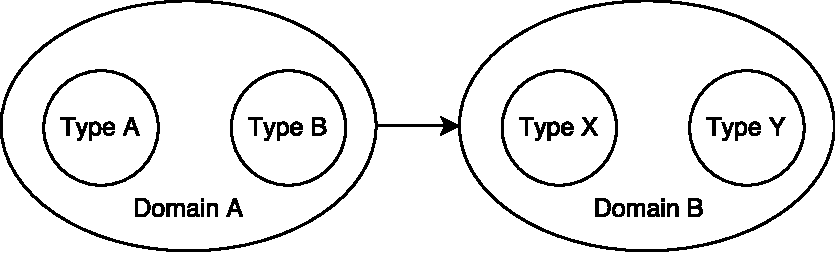
\includegraphics[height=6em]{DA}
  \caption{Domain adaptation}
\end{subfigure}%
\begin{subfigure}{.333\textwidth}
  \centering
  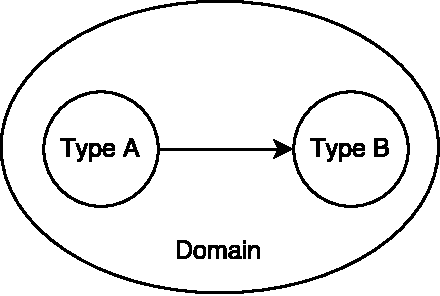
\includegraphics[height=6em]{TL}
  \caption{Transfer learning}
\end{subfigure}
\caption{Difference between domain adaptation and transfer learning.}
\label{fig:da_vs_tl}
\end{figure}

Domain adaptation is also often treated as a sub-topic of transfer learning, as the common definition by \textit{Pan et al.} states: \cite{Pan2010}

\begin{definition}[Transfer learning]\label{def:transfer_learning}
Given a source domain $D_{S}$ and learning task $T_{S}$, a target domain $D_{T}$ and learning task $T_{T}$, transfer learning aims to help improve the learning of the
target predictive function $f(\cdot)$ in $D_{T}$ using the knowledge in $D_{S}$ and $T_{S}$, where $D_{S} \neq D_{T}$, or $T_{S} \neq T_{T}$.
\end{definition}

If the condition $D_{S} \neq D_{T}$ is $true$, Definition~\ref{def:transfer_learning} also applies to domain adaptation, which is treated as a part of transfer learning in this context. In the scope of this paper, \textit{transfer learning} will therefore imply that $D_{S} \equiv D_{T}$ in Definition~\ref{def:transfer_learning}, and \textit{domain adaptation} shall be defined as in Definition~\ref{def:domain_adaptation}:
\newpage
\begin{definition}[Domain adaptation]\label{def:domain_adaptation}
Given a source domain $D_{S}$ and learning task $T_{S}$, a target domain $D_{T}$ and learning task $T_{T}$, transfer learning aims to help improve the learning of the
target predictive function $f(\cdot)$ in $D_{T}$ using the knowledge in $D_{S}$ and $T_{S}$, where $D_{S} \neq D_{T}$.
\end{definition}

In summary, this means that if the application domain changes during the adaptation process, we speak of domain adaptation -- if it does not, usually transfer learning is the more appropriate term (see Figure~\ref{fig:da_vs_tl}). The diverse definitions are mainly based on the unclear definition of the \textit{domain} term, hence it is essential to specify it in each discussion context. The clear definition is not only formally relevant, but also in terms of the used adaptation algorithms, which essentially differ between the two approaches. \cite{Patricia2014}

\section{Applications}
As mentioned above, domain adaptation and transfer learning are particularly interesting if the target domain (or the target data) is unknown at design time and/or expected to change over time. The given examples -- a spam filter for domain adaptation and a product rating analysis for transfer learning -- are most common in research, because they illustrate the topics very well, and are also suitable to demonstrate the differences between the two concepts. Nevertheless, there are several more \textit{real-life} scenarios in which these concepts would fit very well, or even are already in use.

An interesting use case of domain adaptation that is currently investigated in is image recognition in changing visual domains. Since pictures are almost always taken under very different conditions, factors like post, angle and lighting may vary. \textit{Hoffman et al.} presented a classification algorithm that applies domain adaptation principles to this field, and evaluated it with stock images from Amazon as source domain, and real world images as target domain\footnote{\url{https://cs.stanford.edu/~jhoffman/domainadapt}}. \cite{Hoffman2013}

Another field of application for domain adaptation is natural language processing, as shown by \textit{Chan and Ng} in the context of \textit{word sense disambiguation}. WSD is an open topic in natural language processing that describes the problem of detecting the meaning of a word in a specific context (usually a sentence). When changing the domain, e.g. from newspapers to scientific papers, the accuracy of a model trained for WSG operations usually drops because of the different usage of words in different domains. \cite{Chan2007}

\textit{Pan and Yang} also collected an extensive overview about most transfer learning and domain adaptation applications, including (but not limited to) the topics already mentioned above. Due to the shifting usage of the terms domain adaptation and transfer learning in literature, according to the definitions made in section \ref{sec:da-vs-tl}, many examples labeled as \textit{transfer learning} are actually more related to domain adaptation and vice versa in the context of this paper. \cite{Pan2010}

\section{Related concepts}
There are several connected concepts and terms to domain adaptation and transfer learning. Unfortunately, in most cases definitions tend to vary and overlap, as in the case of domain adaptation and transfer learning itself. This sections hence concentrates on the concepts of online and incremental learning and their delimitation of each other, since both topics are highly relevant in the context of concept drift and learning in long time periods. If the concept drift phenomenon affects the domain too, combinations of the described approaches could also become interesting.

\subsection{Online learning}
As described in section \ref{sec:domain-adaptation}, concept drift can have a severe impact on the quality or speed of long-term machine learning applications. Online learning is an option to handle this problem of slowly or abruptly changing input data. While in classic machine learning, a model is trained with one (ideally big) initial learning dataset, in online learning, the model is constantly adjusted to the input data it handles. In most real-life scenarios, this is highly applicable, because data often arrives as a continuous stream (see figure \ref{fig:online-learning}). 

The usual approach to achieve this is to specify some of the parameters of the model that will be altered during the online learning process. Depending on the algorithm used, these may vary, and therefore, this is the most crucial part in designing online learning algorithms (or adapting pre-existing ones). \cite{Gama2014} 

The disadvantage of online learning in the described form is that, due to the fact the all data has to be stored in the memory during the whole execution time, memory consumption tends to be very high. An option to bypass this problem is incremental learning, as described in section \ref{sec:incremental-learning}.

\begin{figure}
	\centering
  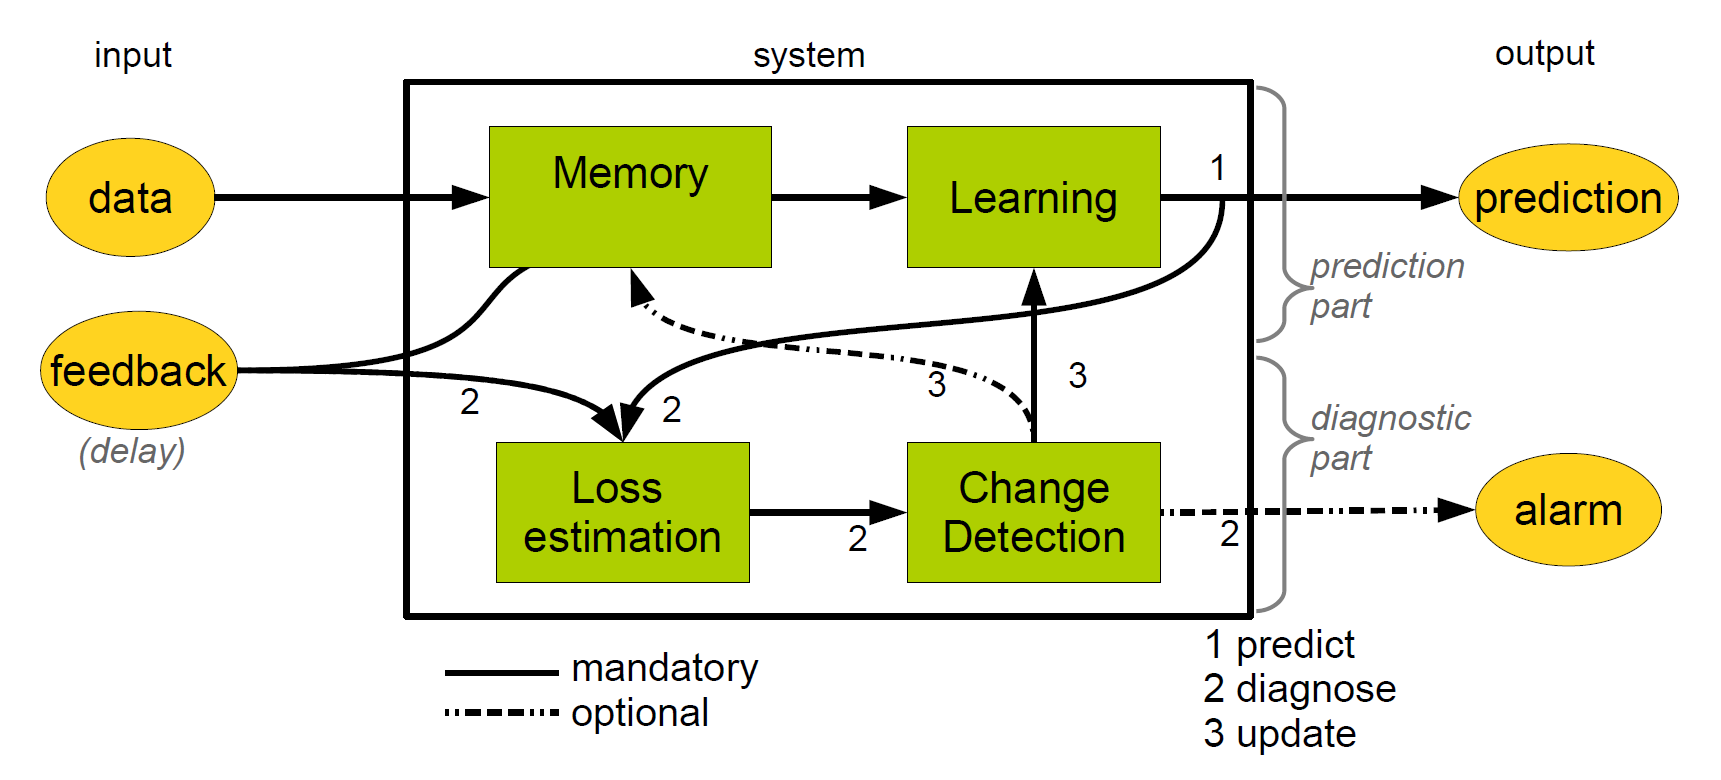
\includegraphics[width=0.9\textwidth]{online-learning}
	\caption{A generic schema for online adaptive learning algorithms. \cite{Gama2014}}
\end{figure}
\label{fig:online-learning}

\subsection{Incremental learning}
\label{sec:incremental-learning}
Since online learning depends on the ability of constantly knowing all previous input data to generate model parameters, it is hardly usable in large datasets -- a problem that has become more and more important due to the high popularity of big data applications and the subsequent collection of enormous amounts of data. Even with modern computational clusters (or \textit{cloud computing}), it is hard and especially expensive to build environments with the required amount of RAM. 

Incremental learning is an approach to circumvent these memory-based limitations of online learning of stream-based input data processing. To achieve this, instead of storing all previously received data fully detailed in the memory, incremental learning algorithms mostly rely on the previously generated models (and some additional meta data). Due to this, it is also possible to react relatively fast, even if the input data is abruptly changing. Working with streams in that way can be way more efficient than distributing the load over many machines, both in costs and in speed -- mainly because it does not repeat the whole model generation process every time it should be adapted. \cite{Gepperth2016}















